\documentclass{article}
\usepackage[utf8]{inputenc}
\usepackage{amsmath,graphicx,varioref,verbatim,amsfonts,geometry}
\usepackage[hidelinks]{hyperref}
\usepackage{listings}
\usepackage[T1]{fontenc}
\usepackage{mathtools}
\usepackage{textcomp}
\usepackage[english]{babel}
\usepackage{wrapfig}
\usepackage{fancyhdr}
\usepackage{amssymb}
\usepackage{enumitem}
\usepackage{xcolor}
\usepackage{lastpage}
\usepackage{graphicx}
\usepackage{matlab-prettifier}
\usepackage{filecontents}
\usepackage{underscore}
\usepackage{makecell}
\usepackage{caption}
\usepackage{subcaption}
\usepackage{siunitx}
\usepackage{mathrsfs}

\pagestyle{fancy}


%% Double underline 
\def\dubline#1{\underline{\underline{#1}}}

%% Matrix
\newcommand\SmallMatrix[1]{{%
		\arraycolsep=0.3\arraycolsep\ensuremath{\begin{pmatrix}#1\end{pmatrix}}}}
	
%% Codeinsert
\definecolor{listinggray}{gray}{0.9}
\definecolor{lbcolor}{rgb}{0.9,0.9,0.9}
\lstset{
	backgroundcolor=\color{lbcolor},
	tabsize=4,
	rulecolor=,
	language=python,
	basicstyle=\scriptsize,
	upquote=true,
	aboveskip={1.5\baselineskip},
	columns=fixed,
	numbers=left,
	showstringspaces=false,      
	extendedchars=true,
	breaklines=true,
	prebreak = \raisebox{0ex}[0ex][0ex]{\ensuremath{\hookleftarrow}},
	frame=single,
	showtabs=false,
	showspaces=false,
	showstringspaces=false,
	identifierstyle=\ttfamily,
	keywordstyle=\color[rgb]{0,0,1},
	commentstyle=\color[rgb]{0.133,0.545,0.133},
	stringstyle=\color[rgb]{0.627,0.126,0.941}
}
\newcounter{subproject}
\renewcommand{\thesubproject}{\alph{subproject}}
\newenvironment{subproj}{
	\begin{description}
		\item[\refstepcounter{subproject}(\thesubproject)]
	}{\end{description}}

\begin{document}
\title{IN3190 - Exam Preparation Questions H23\\
{\Large University of Oslo}}
\author{Daniel Tran}
\date{November 2023}
\fancyhead[L]{Should know to exam H23 - IN3190}
\fancyhead[C]{UiO}
\fancyhead[R]{Daniel Tran}
\cfoot{\thepage\ of \pageref{LastPage}}
\maketitle
\hypersetup{linkcolor=black}
\tableofcontents
\clearpage

\section{Essential Topics}
\subsection{Discrete time}
\subsubsection{Sine, cosine and exponential functions}

    Mathematical formula that establishes the fundamental relationship between the trigonometric functions and the complex exponential function. \newline
    Euler's formula states that for any real number $x$:
    \begin{equation}
        e^{ix} = \cos(x) + i\sin(x)
    \end{equation}
    When $x = \pi$, Euler's formula yields Euler's identity:
    \begin{equation}
        e^{i\pi} + 1 = 0
    \end{equation}
\subsubsection{Elementary discrete signals}
\paragraph{Unit impulse} %Spør gruppelærer om plot fra forelesning
Also known as the dirac delta function.
\begin{equation}
    \delta[n] = \begin{cases}
        1, & n = 0 \\
        0, & n \neq 0
    \end{cases}
    \hspace*{20pt}\text{may also be written as:}
    \hspace*{20pt} \delta[n] = u[n] - u[n-1]
\end{equation}

\begin{figure}[h!]
    \centering
    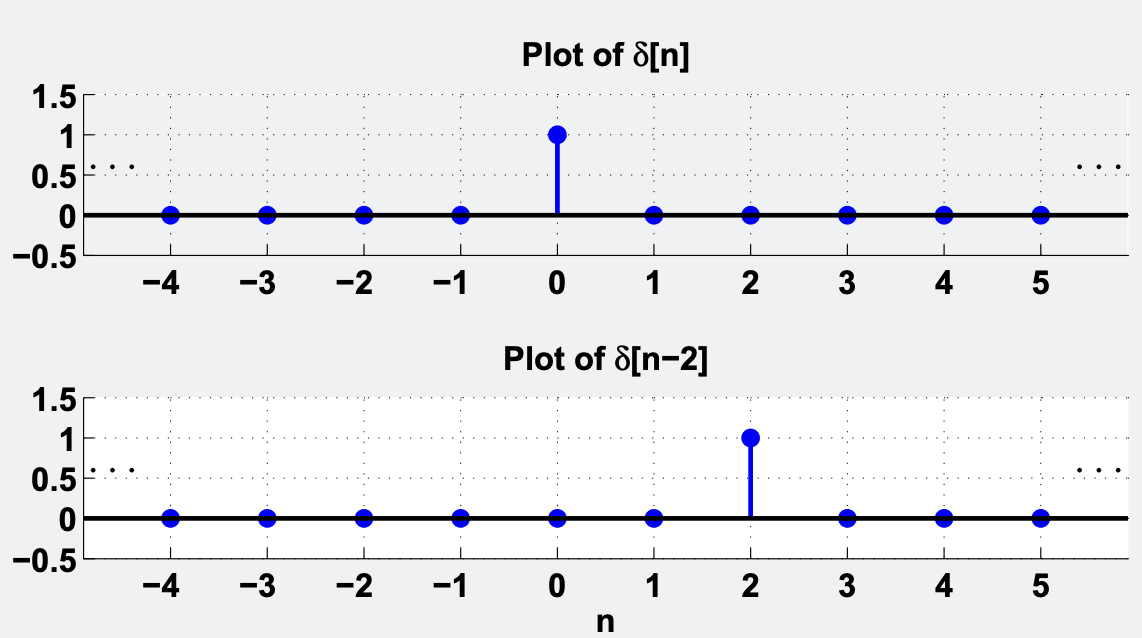
\includegraphics[width=0.5\textwidth]{figures/Discrete time/unit_impulse.png}
    \caption{Unit impulse}
    \label{fig:unit_impulse}
\end{figure}

\paragraph{Step function}
Also known as unit step, unit step function or heaviside function. The value which is zero for negative arguments and one for positive arguments.
\begin{equation}
    u[n] = \begin{cases}
        1, & n \geq 0 \\
        0, & n < 0
    \end{cases}
    \hspace*{20pt}\text{may also be written as:}
    \hspace*{20pt} u[n] = \sum_{k=0}^{\infty} \delta[n-k]
\end{equation}
\begin{figure}[h!]
    \centering
    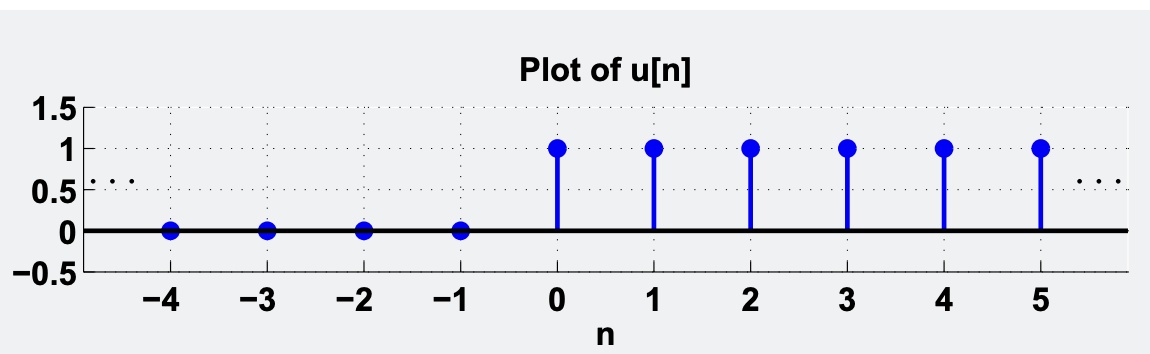
\includegraphics[width=0.5\textwidth]{figures/Discrete time/unit_step_function.png}
    \caption{Unit step function}
    \label{fig:unit_step}
\end{figure}

\newpage
\paragraph{Ramp function}
Also known as the unit-ramp or unit ramp function. Graph shaped like a ramp.
\begin{equation}
u_r[n] = \begin{cases}
    n, & n \geq 0 \\
    0, & n < 0
\end{cases}
\end{equation}
\begin{figure}[h!]
    \centering
    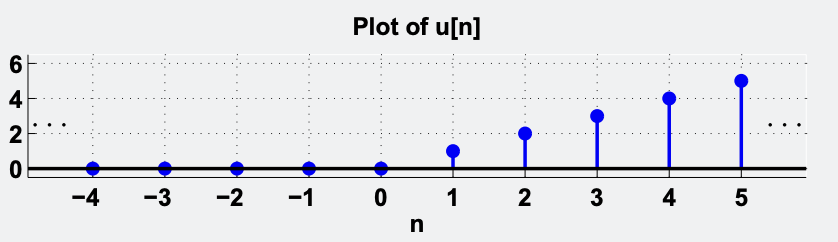
\includegraphics[width=0.5\textwidth]{figures/Discrete time/unit_ramp_function.png}
    \caption{Unit ramp function}
    \label{fig:unit_ramp}
\end{figure}

\paragraph{Periodic sequences} 
$x[n]$ is periodic if and only if $x[n] = x[n+N]$
\begin{itemize}
    \item \textbf{Fundamental period}: 
    \newline Smallest positive integer N which fulfills the relation above
    \item \textbf{Sinusoidal sequences}: 
    \newline $x[n] = A\cos(\omega_0n + \phi)$, where 
    \begin{itemize}
        \item $A$ is amplitude,
        \item $\omega_0$ is the angular frequency
        \item and $\phi$ is the phase of $x[n]$.
    \end{itemize} 
    $x[n]$ is periodic if and only if $\omega_0N = 2\pi k$, for N and k as positive integers.
\end{itemize}

\begin{figure}[h!]
    \centering
    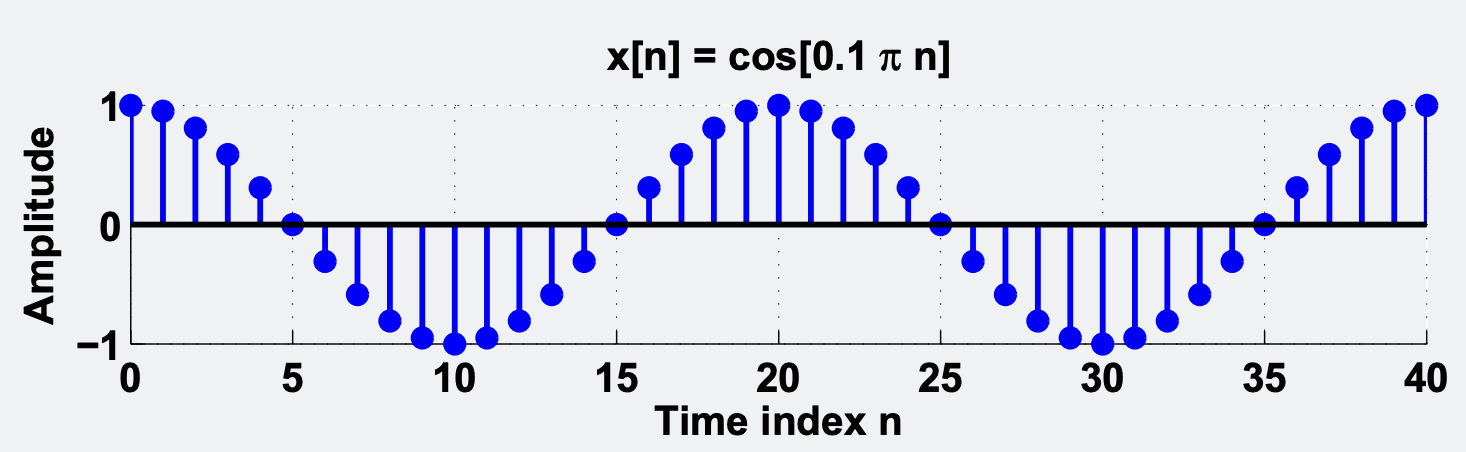
\includegraphics[width=0.5\textwidth]{figures/Discrete time/sinusoidal_sequences.png}
    \caption{Sinusoidal sequences}
    \label{fig:Sinusoidal_sequence}
\end{figure}

\subsubsection{LTI systems, including characteristics via the transformation between input and output}
\paragraph{Linearity:} The relationship between the input $x(t)$ and the output $y(t)$, both being regarded as functions. If $a$ is a constant then the system output to $ax(t)$ is $ay(t)$. Linear system if and only if it $H\{\cdot\}$ is both additive and homogeneous, in other words: If it fulfills the superposition principle. That is:
\begin{equation}
    H\{ax_1(t)+bx_x(t)\} = aH\{x_1(t)\} + bH\{x_2(t)\}
\end{equation}

\paragraph{Time-invariance:} 
A linear system is time-invariant or shift-invariant means that wether we apply an input to the system now or T seconds from now, the output will be identical except for a time delay of S seconds. In other words, if $y(t)$ is the output of a system with a input $x(t)$, then the output of the system with input $x(t-T)$ is $y(t-T)$. The system is invariant becasue the output does not depend on the particular time at which the input is applied.
\\
\\
The fundamental result in LTI system theory is that any LTI system can be characterized entirely by a single function called the system's impulse response $h(t)$. The output of the system $y(t)$ is simply the convolution of the input to the system $x(t)$ with the systems's impulse response $h(t)$.
\\
\\
LTI system can also be characterized in the frequency domain by the system's transfer function $H(s)$, which is the Laplace transform of the system's impulse response $h(t)$. Or Z-transform in the case of discrete time systems.
\begin{figure}[h!]
    \centering
    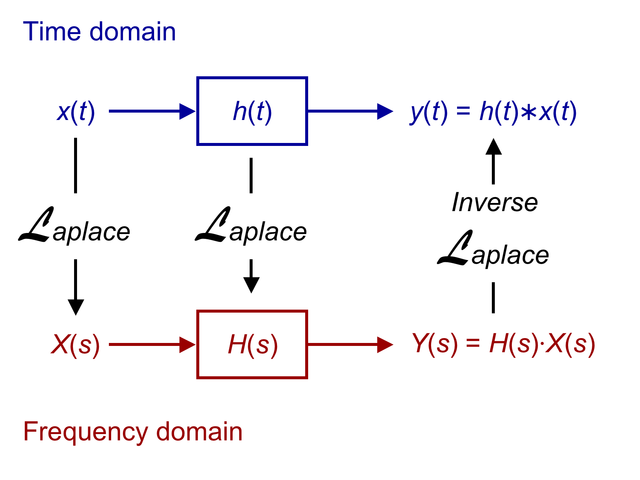
\includegraphics[width=0.5\textwidth]{figures/Discrete time/LTI_time_freq_domain.png}
    \caption{Relationship between the time domain and the frequency domain}
    \label{fig:lti_relationship}
\end{figure}

\subsubsection{Difference equations for system description} %Ask why M
General description of relationship between input x[n] and output y[n] of a LTI system in the time domain (n domain):
\begin{equation}
    y[n] = -\sum_{k=1}^{N}a_ky[n-k] + \sum_{k=0}^{M}b_xy[n-k]
\end{equation}
\begin{itemize}
    \item FIR (finite impulse response): all $a_k = 0$
    \item IIR (infinite impulse response): at least one $a_k \neq 0$
\end{itemize}
The value N represent the order of the difference equation and corresponds to the memory of the system being represented. Because this equations relies on past values of the output, in order to compute a numerical solution, certain past outputs, referred to as the initial conditions, must be known.

\subsubsection{LTI systems written on general summation notation with coefficients and time offsets}

\subsubsection{Casuality}
In control theory, a causal system is a system where the output depens on past and current inputs, but not future inputs. The idea that the output of function at any time depends only on past and present values of input is defined by the property commonly referred to as casusality. 

\subsubsection{Stability and the related convergence for the DTFT}
A linear system is called BIBO (Bounded-input bounded output) stable if its output will stay bounded for any bounded input. 

\paragraph{Discrete-time signals:} For a rational and discrete time system, the conditon for BIBO stability  is that the ROC (region of convergence) of the z-transform includes the unit circle. When the system is causal, the ROC is the open region outside a circle whose radius is the magnitude of the pole with largest magnitude. Therefore, all poles of the system must be inside the unit circle in the z-plane for BIBO stability. For stable systems, the unit circle is part of ROC. 
\\
\\
Causal stable filters have all poles inside $|z| = 1$.

\subsubsection{FIR / IIR}
\paragraph{FIR:}
\subsection{Z-transform}

\subsection{Frequency analysis and DFT}

\subsection{Filter design}

\subsubsection{Advantages/Disadvantages of FIR and IIR filters}
\paragraph{Advantages, FIR filters:}
\begin{itemize}
    \item Can have exact linear phase, which makes h(n) zero points symmetric about $|z| = 1$
    \item  Filter structures are always stable for quantized coefficients.
    \begin{itemize}
        \item Stable IIR filters can become unstable due to rounding errors in coefficients.
    \end{itemize}
    \item Design methods are generally linear. 
    \item Start transient has finite length.
    \item Can be realized efficently in HardWare (but not as efficient as IIR filters)
\end{itemize}

\paragraph{Disadvantages, FIR filters:}


Generally require a higher order than IIR filters to meet the same specifications. This often ensure the FIR filter having greater calculation burden/complexity and larger group delay than the corresponding IIR filter.

\subsubsection{Common ways to design IIR filters}
\begin{itemize}
    \item Specify the filter as a analog/continuous time (CT) equivalent to the dicrete IIR filter you want to design.
    \item Design the analog lowpass filter in continuous time.
    \item Convert the analog lowpass filter to a digital filter using filter transformation.
    \item Convert the digital lowpass filter to the desired filter using a frequency band transformation.
    \item Convert the digital filter to a discrete time (DT) filter (From s-domain to z-domain).
    \item You could also just use an optimization algorithm (e.g. least-square method)
\end{itemize}

\paragraph{Note on standard approximations for IIR filter design:}
Design method involves directly designing the filter coefficients based on a mathematical representation of the desired frequency response. This approach provides more control over the filter characteristics but requires a deeper understanding of filter design principles. The approximation method involves approximating an ideal frequency response by specifying certain filter characteristics, such as filter type, cutoff frequency, and filter order. The goal is to find a set of filter coefficients that can closely match the desired response. Some of the common approximation methods are Butterworth, Chebyshev, and elliptic filters. 

A rough overview of the common method for approximation entails:
\begin{itemize}
    \item Conversion of the digital filter specification to an analog low-pass filter specification
    \item Determination of analog low-pass transfer function $H_a(s)$
    \item Transformation of $H_a(s)$ to the desired digital transfer function $G(z)$
    This method is preferred because:
    \begin{itemize}
        \item Approximation of an analog transfer function is well established and suitable.
        \item Closed expressions for the analog approximation are often obtained.
        \item Large tables for analog filter design are available.
        \item In many cases, digital simulation of an analogue system is sought, i.e. the analogue specification exist.
    \end{itemize}
\end{itemize}



\subsubsection{Typical IIR filters}
When using the approximation method, you have the desired response given as:
\begin{equation}
    |H_d (j\Omega)|^2 = \begin{cases}
        1, & 0 \leq |\Omega| \leq \Omega_c \\
        0, & |\Omega| > \Omega_c
    \end{cases}
\end{equation}

And the approximation as:
\begin{equation}
    |H_c (j\Omega)|^2 = \frac{1}{1 + V^2(\Omega)}
\end{equation}
Where $V^2(\Omega) << 1$ for $|\Omega| \leq \Omega_c$ and $V^2(\Omega) >> 1$ for $|\Omega| > \Omega_c$.

The $V^2(\Omega)$ is called the \textbf{approximation function} and is used to characterize the approximation. Different $V^2(\Omega)$ gives different approximations types.

\paragraph{Butterworth filter:}
\begin{itemize}
    \item $ |H(\Omega)|^2 = \frac{1}{1+\left(\frac{\Omega}{\Omega_c}\right)^{2N}}$, where $N$ is the filter order.
    \item Is flat in the passband, and rolls off towards zero in the stopband.
    \item In a logarithmic plot (bode plot), the response slopes off linearly towards $-\infty$.
    \item Butterworth filters have a monotonically changing magnitude response with frequency $\omega$.
\end{itemize}

\paragraph{Chebyshev filter:}
\begin{itemize}
    \item $|H(\Omega)|^2 = \frac{1}{1 + \epsilon^2 T_N^2 (\Omega / \Omega_c)}$, where $T_N$ is the Nth order Chebyshev polynomial ().
    \item The Chebyshev filter has a ripple in either the passband or stopband, but a steeper roll-off than the Butterworth filter.
    \item Type I Chebyshev filter is an all pole filter and has equiripple (the ripples are of same height) in the passband and a monotonically decreasing stopband.
    \item Type II Chebyshev filter consists of both poles and zeros, with a monotonically decreasing passband and equiripple in the stopband.
\end{itemize}

\paragraph{Elliptic filter:}
\begin{itemize}
    \item $|H(\Omega)|^2 = \frac{1}{1 + \epsilon^2 U_N^2 (\Omega / \Omega_c ) }$, where $U_N(\Omega / \Omega_c)$ is a Jacobian elliptic function.
    \item The elliptic filter has a ripple in both the passband and stopband.
    \item The elliptic filter has both poles and zeros.
    \item Compared to the two other types, the elliptic filter has the narrowest transition band for a given $N$, cutoff frequency $\Omega_p$ and pass/stop-band ripples.
\end{itemize}

\paragraph{A small summary so far:}
Of the prototype analog filters showcased here, \textbf{Elliptic gives best performance in the magnitude-squared response}, but have a highly nonlinear phase response in the passband (Often bad in application). 

\textbf{Butterworth filters} are on the other end with low performance in the magnitude-squared response, but have \textbf{flat magnitude response in the passband and a fairly linear phase in the passband}. They do however require more poles ($N$) to achieve the same stopband specification.


\subsubsection{Common ways to design FIR filters}
These are the ones mentioned in the lecture notes:
\begin{itemize}
    \item \textbf{Window method:} Multiply the ideal impulse response with a window function to get the desired impulse response.
    \item \textbf{Frequency sampling method:} Sample the frequeny response (DTFT) of the desired filter by assuming it to be the DFT. Then use the inverse DFT to get the desired coefficients.
    \item \textbf{Optimization method:} Use algorithms (e.g. Parks-McClellan) or optimization techniques like least squares to iteratively refine the filter coefficients by minimizing the error between the desired and actual frequency response.
\end{itemize}

\subsubsection{Window functions and the consequences of applying them}
Window functions $w(n)$ are of finite lengths and symmetric around their midpoints. 
\begin{equation}
    \underbrace{h(n)}_{\text{Desired filter}} = \underbrace{h_d (n)}_{\text{Ideal filter}} \ast \ w(n)
\end{equation}
Or in the frequency domain:
\begin{equation}
    H(e^{j\omega}) =  H_d (e^{j\omega}) \circledast W(e^{j\omega}) = \frac{1}{2\pi} \int_{-\pi}^{\pi} H_d (e^{j\nu}) W(e^{j(\omega - \nu)}) d\nu
\end{equation}
\begin{figure}[h!]
    \centering
    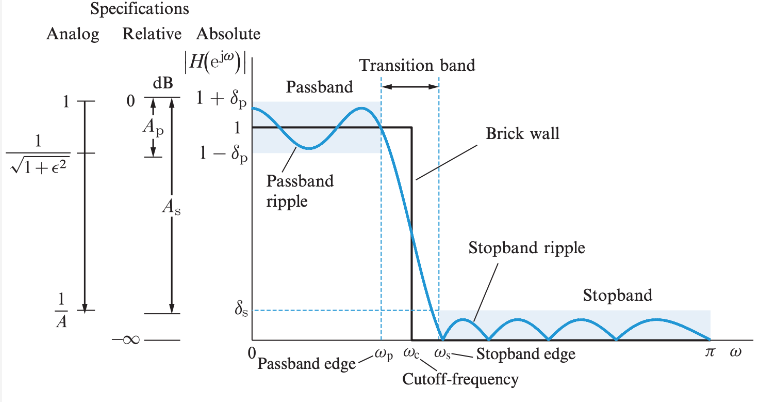
\includegraphics[width=0.75\textwidth]{figures/Filter design/lowpass_tolerance_diagram.png}
    \caption{Example of a lowpass filter tolerance diagram}
    \label{fig:tolerance_diagram}
\end{figure}

How well $H(e^{j\omega})$ approximates $H_d (e^{j\omega})$ is determined by:
\begin{itemize}
    \item The width of the main lobe of $W(e^{j\omega})$
    \item Maximum side lobe level of $W(e^{j\omega})$
\end{itemize}

This method also lacks precise control of $w_p$ and $w_s$.

\paragraph{Some characteristics of window spectrum:}
\begin{itemize}
    \item Pass and stopband ripples are not constant
    \item Stopband level (filter) typically less than peak sidelobe level (PSL) to window. 
    \item PSL, peak passband ripple and passband attenuation $\approx$ independent of $N$.
    \item Width of transition band $\approx$ given by main lobe width window, $F_{WS} \approx C/N$ where $C$ is a constant for each window.
\end{itemize}

\subsubsection{Linear phase and linear-phase filters}
\begin{figure}[h!]
    \centering
    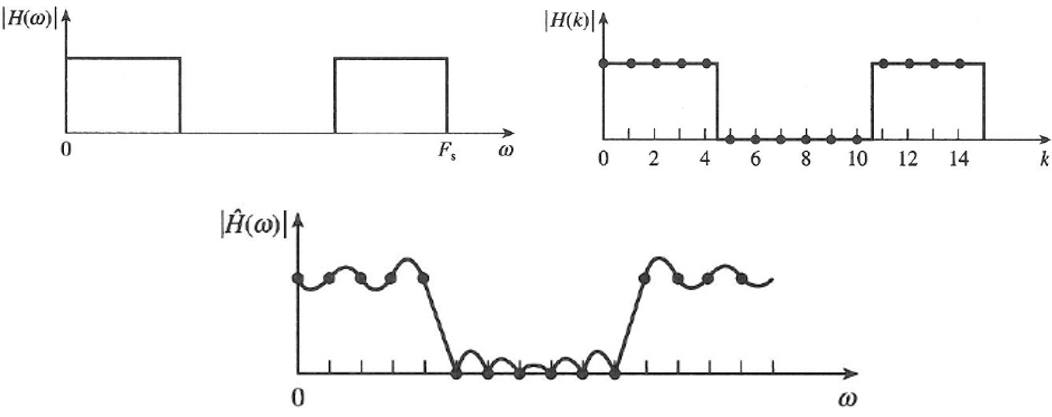
\includegraphics[width=0.75\textwidth]{figures/Filter design/freq_sampling_method.png}
    \caption{Visual representation of the frequency sampling method}
    \label{fig:freq_sampling_method}
\end{figure}

\subsubsection{Grapihcal representation of filter structures and operations}

\subsubsection{Gibb's phenomenon}

\begin{itemize}
    \item Oscillatory behavior in the magnitude response of causal FIR filters found by truncating the filter coefficients of an ideal filter.
    \item If you increase the length of the filter, the number of ripple-peaks will increase in both passband and stopband and the width of these peaks decrease equivalent.
    \item Given the same weighting function, the highest ripple-peak will be unchanged. 
\end{itemize}
\begin{figure}[h!]
    \centering
    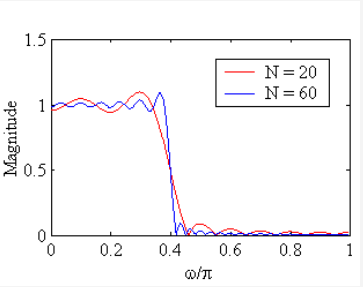
\includegraphics[width=0.75\textwidth]{figures/Filter design/gibbs_effekt.png}
    \caption{Example of Gibb's effect in a lowpass filter}
    \label{fig:gibbs_effect}
\end{figure}

\clearpage

\subsection{Sampling and reconstruction}
\subsubsection{Sampling theorem}
The sampling frequency $\Omega_T = 2\Omega_H$ is called the Nyquist frequency. If this term is satisfied, then the original signal can be recovered from the sampled signal. In practice we often use oversampling (sampling at a higher rate than the Nyquist frequency) to get an appropiate reconstruction.
\subsubsection{Synthesizing an arbitrary signal as a sum of unit impulses}

Sampling corresponds to multiplying with a Dirac comb with distance $T$ between the unit impulses.
In the Fourier domain, this corresponds to convolving with a Dirac comb with distance $F_T$ between
scaled unit impulses. (The distance is $\Omega_T$ if we look at the angular frequency axis)
\begin{figure}[h!]
    \centering
    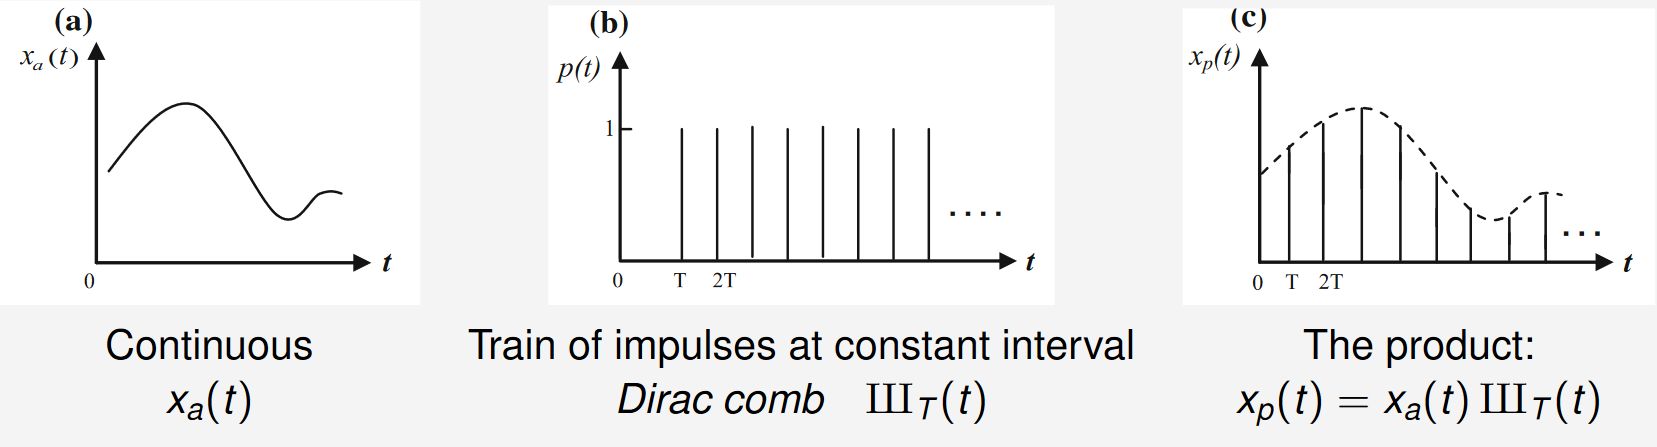
\includegraphics[width=1\textwidth]{figures/Sampling and reconstruction/Sampling_dirac_impulses.png}
    \caption{Sampling with dirac impulses}
    \label{fig:sampling_dirac_impulses}
\end{figure}
\begin{equation}
    x_p (t) = x_a (t) III_T (t) = \sum_{n=-\infty}^{\infty} x_a (t) \delta (t - nT) = \sum_{n=-\infty}^{\infty} x_a (nT) \delta (t - nT) \triangleq x(n)
\end{equation}

\clearpage
\subsubsection{Sampling of band-limited signals}
\begin{figure}[h!]
    \centering
    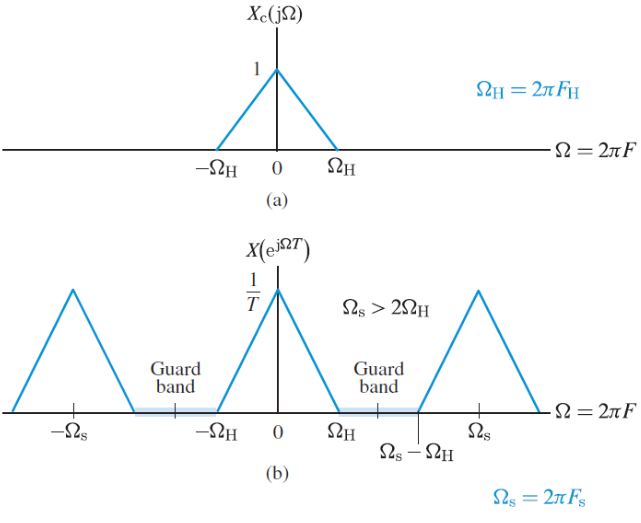
\includegraphics[width=0.75\textwidth]{figures/Sampling and reconstruction/sampling_band_lim_signal.png}
    \caption{Periodic sampling in freq. domain}
    \label{fig:sampling_band_lim_signal}
\end{figure}
The reconstructed signal will repeat itself in the frequency domain. As long the sampling frequency ($\Omega_T$)is equal or greater than the Nyquist rate ($2\Omega_H$), we will be able to seperate the original signal from the aliases. The reconstruction in fig. \ref{fig:sampling_band_lim_signal} can be written as a convolution:
\begin{equation}
    x_r (t) = \sum_{n=-\infty}^{\infty} x_a (nT) g_r (t - nT) 
\end{equation}

Where $g_r (t)$ is the interpolation reconstruction function (I.e. impulse response). The 

\subsubsection{Ideal reconstruction}

The fundamental copy of the Fourier-domain representation of the sampled signal can be found by the 'ideal' filter for the convolution operation is: 
\begin{equation}
    G_r (j\Omega) = \bigg\{ \begin{matrix}
        T, & |\Omega| \leq \Omega_T /2 \\
        0, & |\Omega| > \Omega_T / 2
    \end{matrix}
\end{equation}

This gives the ideal: $X_r (j\Omega) = X_a (j\Omega)$ \\ (Reconstructed Fourier domain representation equals the original Fourier domain representation).

\clearpage
\subsubsection{Upsampling and downsampling}
\begin{figure}[h!]
    \centering
    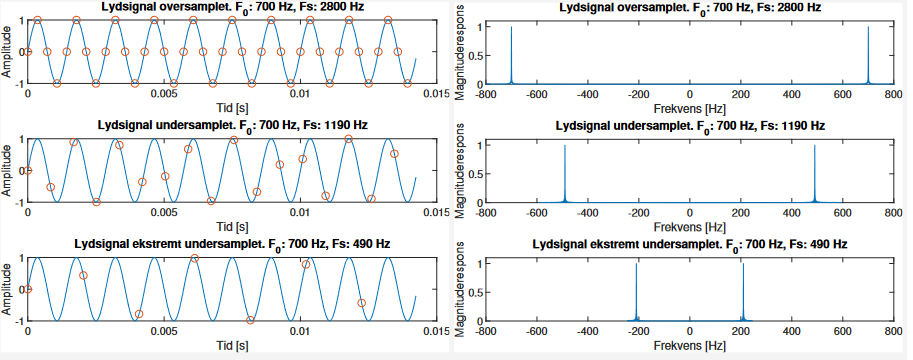
\includegraphics[width=1\textwidth]{figures/Sampling and reconstruction/sampling_examples.png}
    \caption{Example of over/undersampling}
    \label{fig:sampling_example}
\end{figure}

\section{Additional Topics}
\subsection{Discrete time}
\subsubsection{Symmetrical signals}

\subsection{LTI systems and characteristics}

\subsection{Convolution and correlation}

\subsection{Z-transform}

\subsection{Frequency analysis and DFT}

\subsection{Filter design}

\subsection{Sampling and reconstruction}
\end{document}